%\documentclass{article}
\documentclass[journal,12pt,twocolumn]{IEEEtran}
\usepackage{amsmath}
\usepackage{multicol}
\usepackage{enumerate}
\usepackage{amssymb}
\usepackage{iithtlc}
\usepackage{url}
\def\UrlBreaks{\do\/\do-}


\begin{document}
\providecommand{\nCr}[2]{\,^{#1}C_{#2}} % nCr
\providecommand{\nPr}[2]{\,^{#1}P_{#2}} % nPr
\providecommand{\mbf}{\mathbf}
\providecommand{\pr}[1]{\ensuremath{\Pr\left(#1\right)}}
\providecommand{\qfunc}[1]{\ensuremath{Q\left(#1\right)}}
\providecommand{\sbrak}[1]{\ensuremath{{}\left[#1\right]}}
\providecommand{\lsbrak}[1]{\ensuremath{{}\left[#1\right.}}
\providecommand{\rsbrak}[1]{\ensuremath{{}\left.#1\right]}}
\providecommand{\brak}[1]{\ensuremath{\left(#1\right)}}
\providecommand{\lbrak}[1]{\ensuremath{\left(#1\right.}}
\providecommand{\rbrak}[1]{\ensuremath{\left.#1\right)}}
\providecommand{\cbrak}[1]{\ensuremath{\left\{#1\right\}}}
\providecommand{\lcbrak}[1]{\ensuremath{\left\{#1\right.}}
\providecommand{\rcbrak}[1]{\ensuremath{\left.#1\right\}}}
\newcommand{\sgn}{\mathop{\mathrm{sgn}}}
\providecommand{\abs}[1]{\left\vert#1\right\vert}
\providecommand{\res}[1]{\Res\displaylimits_{#1}} 
\providecommand{\norm}[1]{\lVert#1\rVert}
\providecommand{\mtx}[1]{\mathbf{#1}}
\providecommand{\mean}[1]{E\left[ #1 \right]}
\providecommand{\fourier}{\overset{\mathcal{F}}{ \rightleftharpoons}}
%\providecommand{\hilbert}{\overset{\mathcal{H}}{ \rightleftharpoons}}
\providecommand{\system}{\overset{\mathcal{H}}{ \longleftrightarrow}}


\newcommand{\solution}{\noindent \textbf{Solution: }}
\providecommand{\dec}[2]{\ensuremath{\overset{#1}{\underset{#2}{\gtrless}}}}
\newcommand\myeq{\mathrel{\stackrel{\makebox[0pt]{\mbox{\normalfont\tiny def}}}{=}}}

\bibliographystyle{IEEEtran}


\title{ 
%\logo{
Problem Set: Adaptive Filtering
%}
}
%\author{\underline{\textit{Probability, Information measures}}}
\author{U B Desai$^{*}$\thanks{*The author is with the Department of Electrical Engineering, IIT Hyderabad, Kandi 502285.}}
\maketitle

\begin{abstract}
This problem set covers all the
basic concepts in Adaptive Filtering.
\end{abstract}


\section{Some Basic Problems in Estimation and Matrix Computation}

\begin{enumerate}
\item Consider the following M-th order FIR adaptive structure for noise cancellation shown in class
\begin{figure}
\centering
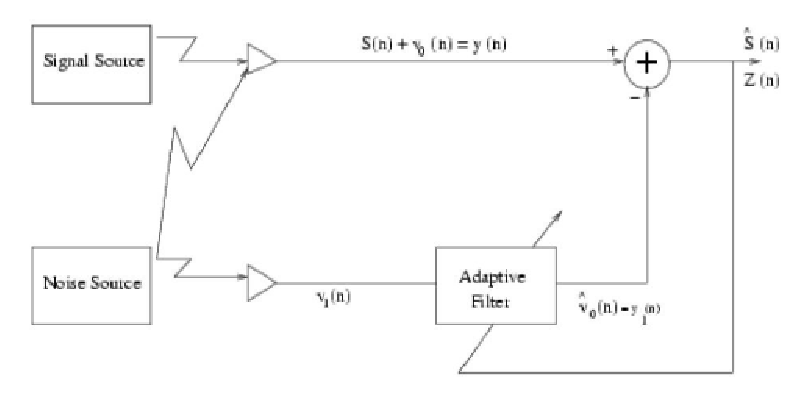
\includegraphics[width=\columnwidth]{./figs/figure1.eps}
\caption{}
\label{fig:hw1}
\end{figure}


Assume that $v_i(n)$ and s(n) are statistically independent.Let $e(n)=s(n)+v_0(n)-\hat{v}_0(n)$.Now suppose the adaptation rule is chosen such that $E[e^2(n)]$ is minimized.Then show that $E[e^2(n)]=E[(s(n)-\hat{s}(n))^2]$.Thus minimizing $E[e^2(n)]$ will indeed yield $\hat{s}(n)$ as the minimum mean sqaure estimate of s(n).

\item Let $\{\large{y}_k\}_{k=1}^N$ be N measurements of unknown constant c. The problem is to derive the expression for the $l_2$,$l_1$, and $l_\infty$ estimate of the constant c using the measurements $\{\large{y}_k\}_{k=1}^N$\\
We model the measurements as sample values of a discrete time random variable Y having the density function\\
                            $$f_Y(y)=\quad\sum_{k=1}^{N}{\alpha_k}{\delta(y-y_k)}$$
                             
where $\alpha_k$ are such that $\quad\sum_{k=1}^{N}{\alpha_k}=1.$\\
Show that
\begin{enumerate}[(a)]
\item The $l_2$ estimate of c is given by
$$\hat{c}=\quad\sum_{k=1}^{N}{\alpha_k}{y_k}$$
\item The $l_1$ estimate of c is given by $\hat{c}={y_p}$, for $1\leq{p}\leq{N}$ such that
$$\quad\sum_{y_k<{\hat{c}}}\alpha_{k}=\quad\sum_{y_k>{\hat{c}}}\alpha_{k}$$

\item The $l_\infty$ estimate is given by
$$\hat{c}=\frac{min\{{y_k}\}+max\{y_k\}}{2}$$
\end{enumerate}
\item Consider the problem of estimating the mean and variance of a Gaussian distributed random variable.\\

Let
$${X_k}, {k=1},... N$$\\
be N independent samples of a stationary Gaussian distribution.Thus\\
$$f_{{X_k}|{M},{V^{{(x_k}|m,{\sigma^2})}}}=\frac{1}{2\pi\sigma^2}e^{-(x_k-m)^2/(2\sigma^2)}$$
and letting $Z=\{{X_1},...,{X_N}\},z=\{x_1,...,x_n\}$
$$f_{{Z|M},{V^{{(z|m,\sigma^2})}}}=\prod_{k=1}^{N}f_{{X_k}|{M},{V^{{(x_1}|m,{\sigma^2})}}}=\frac{1}{(2\pi\sigma^2)^{N/2}}exp[-\quad\sum_{k=1}^{N}{({x_k}-m)^2}/{2\sigma^2}]$$
\begin{enumerate}[(a)]
\item Assume $\sigma^2$ is known. Show that the MLE of m is given by
$$\hat{m}_{MLE}=\frac{1}{N}\quad\sum_{k=1}^{N}x_{k}$$\\
and that is an unbiased estimate.
\item Assume m is known. Show that MLE of  $\hat{\sigma^2}$ is given by
$$(\hat{\sigma^2})_{MLE}=\frac{1}{N}\quad\sum_{k=1}^{N}({x_k}-m)^2$$\\
and that is unbiased.
\item\textit{Neither m nor $\sigma^2$ is known.} Show that
$$\hat{m}_{MLE}=\frac{1}{N}\quad\sum_{k=1}^{N}x_{k},  (\hat{\sigma^2})_{MLE}=\frac{1}{N}\quad\sum_{k=1}^{N}({x_k}-\hat{m}_{MLE})^2$$\\
Furthermore show that, $\hat{m}_{MLE}$ is unbiased, while $(\hat{\sigma^2})_{MLE}$ is biased with\\
$$E[(\hat{\sigma^2})_{MLE}]=\frac{N-1}{N}\sigma^2$$
\item Recursive computation of $\hat{m}_{MLE}$ and $(\hat{\sigma^2})_{MLE}$.Show that if $\hat{m}_{MLE}:=\hat{m}_{N}$ and $(\hat{\sigma^2})_{MLE}:=(\hat{\sigma^2})_{N}$ then
$$\hat{m}_{N}=\frac{1}{N}[(N-1)\hat{m}_{N-1}+x_{N}]$$\\
$$\hat{\sigma^2}_{N}=\frac{1}{N}[(N-1)\hat{\sigma^2}_{N-1}+\frac{N}{N-1}(x_{N}-m_{N})^2]$$
\end{enumerate}

\item Solve the following $l_2$ minimization problems.

\begin{enumerate}[(a)]
\item Let A be an m $\times$ n matrix, x an n $\times$ 1 vector, and y an m $\times$ 1 vector. Find x such that\\
$${\|A{x}-y\|}^2 =(A_{x}-y)^T(A_{x}-y)$$\\
is minimized.\\
\item Let A be an m $\times$ n matrix, x an n $\times$ 1 vector, and y an m $\times$ 1 vector. Find x having minimum $l_2$ norm $({\|{x}\|}^2=x'x$) and satisfying $Ax=y$; ie.
$$ \quad\min_{subj.Ax=b}{\|{x}\|}^2$$\\
Note: These are two fundamentals finite dimensional $l_2$ approximation problems which can serve as prototypes for any other finite dimensional $l_2$ approximation problem.
\end{enumerate}
\item \textbf{On QR Decomposition}\\
\textit{Definition:}LetA be an m$\times$n matrix with m$>$n and rank p; then the QR decompositon of A is defined by\\
\begin{align*}
A=\begin{bmatrix}Q & N\end{bmatrix}
\begin{bmatrix}R_1&R_2\\0&0\end{bmatrix}\begin{bmatrix}QR_1&QR_2\end{bmatrix}&\myeq QR\\
\end{align*}
where
\begin{enumerate}[(a)]
\item the dimensions of various matrices are Q:m$\times$p, N:m$\times(m-p)$,$R_1:p\times$p,$R_2:p\times(n-p).$
$R=\begin{bmatrix} R_1&R_2\end{bmatrix}$ is p$\times$ n.
\item $\begin{bmatrix}Q&N\end{bmatrix}$ is an orthogonal matrix,namely ,
$$\begin{bmatrix}Q&N\end{bmatrix}
\begin{bmatrix}Q^T\\N^T\end{bmatrix}=I_m=\begin{bmatrix}Q^T\\N^T\end{bmatrix}
\begin{bmatrix}Q&N\end{bmatrix}$$
Note the obvious $QQ^T\neq I$ and $NN^T\neq I$. But $Q^TQ=I_{p}$ and $N^TN=I_{m-p}.$
\item $R_1$ is a p$\times$p upper triangular matrix.\\
Note, if p=n then $R_2=0.$
\end{enumerate}
\begin{enumerate}[(a)]

\item Show that the columns of Q provide an orthogonal basis for the range space of A, while the columns of N provide an orthogonal basis for the null space of $A^T$.
\item\textbf{Algorithm for obtaining the QR Decomposition}\\
Consider a 2$\times$1 column vector $\begin{bmatrix}
x&y\end{bmatrix}^T.$ Now it is shown earlier that the orthogonal Givens rotation
\begin{align*}
G=\begin{bmatrix}c&s\\-s&c\end{bmatrix},
c=\frac{x}{\sqrt{x^2+y^2}}\\s=\frac{y}{\sqrt{x^2+y^2}}
\end{align*}
when applied to $\begin{bmatrix}x&y\end{bmatrix}^T$,yields
$$G\begin{bmatrix}x\\y\end{bmatrix}=\begin{bmatrix}
\sqrt{x^2+y^2}\\0\end{bmatrix}$$
First figure out how the above method can be used to selectively zero elements of any column vector.Using this idea develop an algorithm for computing the QR decomposition of an m$\times$n $(m> n)$ matrix A. You can illustrate your algorithm by considering a full rank 4$\times$3 matrix A.
\end{enumerate}
\item One possible norm for an m$\times$n matrix A is defined as
\begin{align*}
\|A\| &\myeq \quad\max_{x^Tx=1,x\varepsilon\Re^n}{(x^TA^TAx)}
\end{align*}

Now let the SVD of an m$\times$n matrix A be A=U$\Sigma{V^T}.$Show that $\|A\|=\sigma_{max}(A)$.
\item Let the SVD of an m$\times$n matrix A be A=U$\Sigma{V^T}.$Now define the pseudo inverse of A as
$$A^\dagger=V\Sigma^{-1}U^{T}$$\\
verify that the above $A^\dagger$ satisfies the following identities for the matrix to be a pseudo inverse.
%{\scriptsize
\begin{enumerate}[(i)]
\begin{multicols}{2}
\setlength{\itemsep}{1em}
\item ${(A^\dagger)}^\dagger=A,$
\item ${(A^T)}^\dagger={(A^\dagger)}^T,$
\item ${A^\dagger}{AA^\dagger}=A^\dagger,$
\item $A{A^\dagger}A=A,$
\item $({A^\dagger}A)^T={A^\dagger}A,$
\item $A^\dagger={({A^T}A)^\dagger}{A^T},$
\item $A^\dagger=A^T{(A{A^T})}^\dagger.$
\end{multicols}
\end{enumerate}
%}
\end{enumerate}

\section{Levinson's Algorithm}
\begin{enumerate}
\item\textbf{Computing the Sample Covariance Matrix}\\
\smallskip
Let $Y(k)$ be a discrete time stochastic process, and $\{y(k)\}_0^{N-1}$ be a realization of this process.\\

A typical problem in practice is to compute the second order statistics of the process.\\
\smallskip
The procedure for computing the mean is well known; in fact it is the answer obtained earlier
using the maximum likelihood estimation procedure under Gaussian assumption, namely
\bigskip
\bigskip
$$\hat{m}_N=\frac{1}{N}\quad\sum_0^{N-1}Y(k)$$\\
\bigskip
To avoid a new notation we use the \textit{computer programming definition}\\
\bigskip
\bigskip
$Y(k):=Y(k)-\hat{m}_N\rightarrow y(k):=y(k)-\hat{m}_N$\\
\bigskip
Now we look for procedures for computing the covariance of Y(k) using $\{y(k)\}_0^{N-1}.$
\begin{enumerate}[(a)]
\item Let\\
\bigskip
$$\bar{r}_N{(k)}=\frac{1}{N-k}[{\quad\sum_{j=0}^{N-k-1}}{y(j+k)}y(j)], k=0,1,...N-1 $$\\
show that\\
\begin{enumerate}[i.]
\item $\bar{r}_N{(k)}$ is an unbiased estimate of the true covariance parameter $r(k)=E[(j+k)Y(j)]$
\item the covariance matrix constructed using $r_N{(k)}$ will not be non-negative definite. Because of this problem one looks for alternative methods for computing the sample
covariance matrix.
\end{enumerate}
\item Alternately let the sample covariance matrix be defined as
$$r_N{(k)}=\frac{1}{N-k}[{\quad\sum_{j=0}^{N-k-1}}{y(j+k)}y(j)], k=0,1,...N-1 $$\\
\begin{enumerate}[i.]
\item Show that $r_N{(k)}$ is not an unbiased estimate of the true covariance parameter; nevertheless it is an asymptotically unbiased estimate.
\item Show that the covariance matrix constructed using $\bar{r}_N{(k)}$ is non-negative definite.\\
(Hint: Express the sample covariance matrix as a product of data matrix with its
transpose).\\
\end{enumerate}
\end{enumerate}
\bigskip
\item Let $x(\cdot)$ and $y(\cdot)$ be discrete time, jointly stationary zero mean processes with $E[x(n)y(m)]=r_{xy}(n-m),E[y(n)y(m)]=r_{yy}(n−m)$ Show that the parameters involved in computing the following linear least-squares estimates are identical.
\begin{enumerate}[(a)]
\item $\hat{E}[x(n)|y(n-1),...y(n-M)]$\\
\bigskip
\item $\hat{E}[x(n+N)|y(n+N-1),...y(n+N-M)]$ \\
\bigskip
\textit{Note:}This simple result shall be used often.
\end{enumerate}
\bigskip
\bigskip
\bigskip
\item \textbf{Determining $\hat{x}(k|n)$ using Levinson’s Algorithm}\\
\smallskip
In class we developed the Levinson’s Algorithm for the one step prediction problem and for generating the innovations. In this problem you are required to develop a recursive scheme for
computing $\hat{x}(k|n)$ in the framework of Levinson’s algorithm.\\
Show that\\
\bigskip
$\hat{x}{(k|n+1)}=\hat{x}(k|n)+\Gamma(k,n)\epsilon(n)$\\
Determine the expression for the gain $\Gamma(k,n)$ and an expression for recursively computing it.
The above is referred to as the measurement update equation.\\
\bigskip
\item In the Levinson Algorithm derive the expression
$$p(n)=r(0)+\quad\sum_{i-0}^{n-1}{a_n(n-i)r(i-n)}$$\\
where $p(n)$ is the innovations (error) variance
$$p(n)=E[\{y(n)-\hat{y}(n|n-1)\}^2]$$
\item Let $y{(\cdot)}$ be a zero mean process with
$$E[y(k+m)y(m)]=(\frac{1}{4})^{\vert{k}\vert}$$\\
\medskip
and $x(\cdot)$ be another process with\\
\bigskip
$E[y(k+m)y(m)]=\begin{cases}
\bigskip
(2/3)^k& k \geq 0\\
(1/3)^k& k\leq 0\\
\end{cases}$\\
\bigskip
$E[x(k+m)x(m)]=(\frac{1}{2})^{\vert{k}\vert}$\\
\medskip
\begin{enumerate}[(a)]
\item Find the optimal filter for computing the linear least squares estimate of $x(n + N ), N > 0,$
based on $\{y(k),k\leq n \}.$
\end{enumerate}
\item \textbf{Simulation:}Consider the sample values of a stationary process y(·) on the home page for the\\
 \textbf{ASP course:}in http$://$sharada.ee.iitb.ac.in$/$ ee608$/,$ file name is levinson.dat
\begin{enumerate}[(a)]
\item Determine the first 50 covariance lags $r(n)$   ${0}\leq {n} \leq {50}.$
\item Using Levinson’s algorithm determine an appropriate AR model. Comment on the goodness
of this model. If there are any deficiencies or problems give reasons for them.
\end{enumerate}
\end{enumerate}
\section{}
\begin{enumerate}
\item Consider the state space model
$$X(k+1)=F(k)X(k)+G(k)u(k),    x(0)=x_{0}$$\\
with $E[X_0]=0, E[u(k)]=0, E[x_{0}{x_{0}}^T]=\Pi_{0}, E[u(k)u^T(j)]=Q(k)\delta(k-j),$ and for $j \geq {k},E[x(k)u^T(j)]=0.$ 
Let $\Pi(k)=E[x(k)x^T(k)].$   
\bigskip
\begin{enumerate}[(a)]
\item Show that\\
$$\Pi(k+1)=F(k)\Pi(k){F^{T}(k)}+G(k)Q(k)G^T(k)$$\\
\bigskip
\item Show that\\
$$\Pi(k)-P(k\vert{k-1})\geq {0}$$\\
\bigskip
Give an interpresentation to this result.
\end{enumerate}
\medskip
\item Verify the matrix inversion identity
$${(A+BCD)^{-1}}=A^{-1}-A^{-1}B{(C^{-1}+D{A^{-1}}B)}^{-1}DA^{-1}$$
\medskip
\item Show that the filtered error covariance matrix is given by\\
\medskip
$$P(k \vert k)=P(k \vert {k-1})-P(k \vert {k-1})H^T{R_\epsilon}^{-1}(k)HP(k \vert {k-1})$$\\
\item \textbf{Measurement Update and Time Update in Kalman Filtering}\\
Let the filtered estimate be ${\hat{x}(k \vert k)}\myeq {\mathcal{P}}(k) \vert \{y(0),... y(k)\}].$ Using the kalman Filter (one step predictoer) equations developed in class and associated manipulations, show that the filtered and one step predicted estimate can be computed through the following equations.\\
\smallskip
\textit{Measurement Update} 
\bigskip
\begin{align*}
\hat{x}(k \vert k )& =\hat{x}(k \vert (k-1)+K_f(k)[y(k)-H\hat{x}(k\vert {k-1})], \hat{x}(0\vert {-1})=0\\
k_f(k)& =P(k\vert{k-1})H^T{R\epsilon}^{-1}(k)\\
&=P(k\vert k)H^TR^{-1}\\
R_\epsilon(k)& =R+HP(k\vert {k-1})H^T\\
P(k\vert k)& =P(k\vert {k-1})-P(k\vert{k-1})H^T{R_\epsilon}^{-1}HP(k\vert {k-1}), P(0\vert {-1})=0
\end{align*}
\textit{Time Update}
\bigskip
\begin{align*}
\hat{x}({k+1}\vert k) &=F{\hat{x}}(k \vert k)\\
P({k+1}\vert k) &=FP(k \vert k)F^T+GQG^T\\
\end{align*}
\medskip
Note, form the above equation it should be obvious as to why the computation of the filtered estimate from the one step predicted estimate is referred to as the Measurement Update, while the computation of the one step predicted estimate from the filtered estimate is referred to as the Time Update. 
\end{enumerate}
\section{}
\begin{enumerate}
\item Find an expression for $J_{min}$, the Wiener optimal cost.\\
\medskip
\item \textit{Method of Steepest Descent:}\\
\smallskip
In class we derived the LMS algorithm using the method of, what was referred to as, \textit{gradient descent}.In literature, the method of steepest descent is talked about very often. Most of the steps in the method of gradient descent and steepest descent are the same, except for the selection of the step size parameter $\mu $. In the method of steepest descent, one solves another minimization problem for selecting $ \mu.$ This is illustrated in the present problem.\\
\smallskip
Consider the Problem\\
$$\quad\min_W{J(n)}=\quad\min_W\{E[(d(n)-W^TX(n))^2]\}$$\\
\medskip
with notations and assumptions as defined in class. This problem can be solved non-iteratively, by using the orthogonality principle or simply differentiating the above. On can obtain an iterative algorithm using the method of steepest descent. We define the steepest descent based iterative equation as\\
$$W(n+1)=W(n)+\mu(n){(-\nabla}_W[J(n)])$$\\
\medskip
Now $\mu$ is selected such that $\bar{J}(n)=[J(n)]_{W=W(n+1 )}$ is minimized w.r.t $\mu.$ Show that that the optimal value of Show that that the optimal value of $\mu$ is given by is given by
$$\mu(n)=\frac{(\nabla_{W_{(n)}}[\bar{J}(n)])^T(\nabla_{W_{(n)}}[\bar{J}(n)])}{(\nabla_{W_{(n)}}[\bar{J}(n)])^TR(\nabla_{W_{(n)}}[\bar{J}{(n)}])} $$\\
\medskip
Note that, here $\mu $ is time varying.
\medskip
\item In class we showed that the LMS algorithm converges in the mean if $\mu $ is selected such that $0<\mu <2{\lambda}_{max}.$ \\
Show that this condition is satisfied if $\mu$ is selected such that $0 < \mu < 2/(M$ (signal power)).\\
\bigskip 	
\textbf{Simulations}
\medskip
\item Using the data given to you in Problem Set 2, implement the LMS algorithm in the predictive mode to whiten the given process. You will need to select an appropriate order for the filter.\\
What is the eigenvalue spread for this data set?\\
\textit{Remark:}
The data given earlier in Problem Set 2 was generated from a four pole – three zero model:\\
$$H(z)= \frac{1+{0.5z^{-1}}+0.007z^{-2}-0.013z^{-3}}{1-1.2z^{-1}+0.575z^{-2}-0.1375z^{-3}-0.0125z^{-4}}$$
driven by uniform white noise. This was deliberately done to violate various assumptions that we have been making and still see the validity of different adaptive algorithms.
\medskip
\begin{enumerate}[(a)]
\item Generate the data for LMS algorithm using the model\\
$$H(z)= \frac{(z-0.8)(z+0.7)}{(z-0.9)(z+0.8)(z+65)}$$\\
\bigskip
To generate the data you will drive the above system by a Gaussian white process with zero mean and variance preselected by you. Determine how long you need to run the system, so that it has reached steady state. Once in steady state, start collecting the data. Collect, at least, 512 points (you may need more in case your LMS algorithm is going to take a long time for convergence).
\smallskip
\item Get an estimate for the signal energy for the above data, and using this estimate determine the range for $\mu.$ 
Select two values for $\mu$ in this range.
\item Run the LMS algorithm in the predictive mode for the data that you have generated and for the two choices of $\mu.$
\item Do a validation test. You should use the following for the purpose of comparison
\end{enumerate}
\begin{enumerate}[i.]
\item Learning curve (i.e mean square error curve)\\
\item Convergent values of $W(n)$\\
\item Whiteness of the error\\
Comment on which choice of $\mu$ gives better results, and why.
\end{enumerate}
\end{enumerate}
\section{}
\begin{enumerate}
\item \textit{Complex LMS Algorithm}\\
Let all the variables in the algorithm be complex. Now, wherever  you have transpose terms like $A^T$, it will get replaced by $A^H={(A^*)}^T$. Let\\
\begin{align*}
&\text{Tap input vector be X(n)}={X_R}(n)+j{X_I}(n)\\
&\text{Desired Response be d(n)}={d_R}(n)+jd_I(n)\\
&\text{Tap Weight Vector be W(n)}={W_R}(n)+j{W_I}(n)\\
&\text{Estimation Error be e(n)}=e_R(n)+j{e_I}(n)\\    
\end{align*}
\medskip
Show that
\begin{align*}
W_R(n+1)& ={W_R}(n)+\mu[e_R(n)X_R(n)-e_I(n)X_I(n)]\\
W_I(n+1)& =W_I(n)+\mu[e_R(n)X_I(n)+e_I(n)X_R(n)]\\
\end{align*}
where
\begin{align*}
e_R(n)& =d_R(n)-W_{R}^{T}{X_R(n)}+W_{I}^{T}(n)X_I(n)\\
e_I(n)& =d_I(n)-W_{R}^{T}{X_I(n)}-W_{I}^{T}(n){X_R(n)}\\
\end{align*}
\smallskip
Note: You will need to use derivative of complex quantities w.r.t to real and imaginary parts.\\
Let $f(W)$ be a scalar complex function of a complex column vector $W=W_R+jW{_I},$and $W_R=[w_{R}^{1}...w_{R}^{M}]^T,W_I=[w_{I}^{1}...w_{I}^{M}]^T.$ Now the derivative of $f(W)$ w.r.t W is defined as:
\bigskip
\begin{align*}
\frac{\partial{f(W)}}{\partial{W}}=\begin{bmatrix}{\frac{\partial{f(W)}}{\partial{w}_R^1}}-{j\frac{\partial{f(W)}}{\partial{w}_I^1}} \\[12pt]
{\frac{\partial{f(W)}}{\partial{w}_R^2}}-{j\frac{\partial{f(W)}}{\partial{w}_I^2}} \\
\vdots \\
{\frac{\partial{f(W)}}{\partial{w}_R^M}}-{j\frac{\partial{f(W)}}{{w}_I^M}}
\end{bmatrix}
\end{align*}
and the conjugate derivative is defined as\\
\begin{align*}
\frac{\partial{f(W)}}{\partial{W}^{*}}=\begin{bmatrix}{\frac{\partial{f(W)}}{\partial{w}_R^1}}+{j\frac{\partial{f(W)}}{\partial{w}_I^1}} \\[12pt]
{\frac{\partial{f(W)}}{\partial{w}_R^2}}+{j\frac{\partial{f(W)}}{\partial{w}_I^2}} \\
\vdots \\
{\frac{\partial{f(W)}}{\partial{w}_R^M}}+{j\frac{\partial{f(W)}}{{w}_I^M}}
\end{bmatrix}
\end{align*}
\bigskip
\item \textbf{Simulation:}This problem deals with \textit{adaptive noise cancellation} using the LMS algorithm. You will need two data streams: one corresponding to signal plus noise and the other corresponding to noise. You could synthesize such
data but this would be too far from the real situation. Thus
\medskip
\begin{enumerate}[(a)]
\item Use the speech data files provided on the course web page.\\
\smallskip
The files are for speech plus noise, and only noise. You will notice that you cannot decipher the speech when you play the speech plus noise file; but upon proper implementation of the noise cancellation algorithm you will be able to decipher the speech.
\begin{enumerate}[i.]
\medskip
\item noise3.wav and signal noise3.wav form one par
\item snp.wav and n.wav from one pair
\item look for other such pairs on the web; these can also be included in the noise cancellation simulation data
set.
\end{enumerate}
\bigskip
\item OR (optional) your group should capture its own data streams.\\
You need to generate one stream as: speech data plus noise, and the other stream as only noise. You could
use two microphones to capture the data streams. The main catch is in capturing both the data streams simultaneously.\\
Have at least two set of data; each with a different SNR (one with low SNR and the other with high SNR).
\end{enumerate}
\end{enumerate}
\section{}
\begin{enumerate}
\item \textit{An alternate aspect of the convergence analysis for the RLS algorithm}\\
Suppose there exists a true model for $d(n)$ of the form\\
$$d(n)=X^T(n)W_o+v(n)$$\\
where $v(n)$ is some unknown error, and $W_o$ the true weight vector which is also unknown.\\
\medskip
The question we want to investigate is whether $W(n)\rightarrow {W}_o$ in the mean and the mean square sense. Note this is different from what we did in class where we were considering the convergence of $W(n)$ to $W_*$ the Wiener optimal
solution.\\
\medskip
In this problem we shall only investigate the convergence of $W(n) to W_o$ in the mean. Also consider the RLS
algorithm based on
$$W(n)=[\quad\sum_{k=0}^{n}X(k)X^T(k)]^{-1}[\quad\sum_{k=0}^{n}X(k)d(k)]$$\\
\begin{enumerate}[(a)]
\item Show that, if ${v(i)}\perp\!\!\!\perp{X(k)}$for $k \leq i$, then $E[W(n)] = W_{o}.$\\
\medskip
\item In a deterministic sense, show that $W(n)\rightarrow W_o$ if $\lim_{n\to\infty}\frac{1}{n}\sum_{k=0}^{n}X(k)v(k)=0.$\\
\end{enumerate}
\item Start with the following non-recursive equations and derive the RLS algorithm having the necessary initial condition $(P(0)=\delta^{-1})I.$\\
$$W(n)=[\delta I+\quad\sum_{i=1}^{n}X(i) X^T(i)]^{-1}[\quad\sum_{i=1}^{n}X(i)d(i)]$$\\
$$P(n)=[\delta I+\quad\sum_{i=1}^{n}X(i)X^T(i)]^{-1}$$\\
\item Simulate the normalized LMS algorithm and compare with the LMS algorithm. For this you should use the 
\begin{enumerate}[(a)]
\item data generated by the model in the previous problem.
\item generate the data for an AR model\\
$$x(n)+a_1{x}{(n-1)}a_2{x}{(n-2)}a_3{x}{(n-3)}+a_4{x}{(n-4)}=v(n)$$\\
where the AR parameters correspond to the four poles $\lambda_1=0.8,\lambda_2=0.6 +j{0.5},\lambda_3=0.6−j{0.5},\lambda_4= 0.65.$ We
assume that that $v(n)$ is zero mean, unit intensity white sequence. You will need to determine the AR parameters for
the given pole locations. Note, you should generate at least 100 data sets, each data set having large enough points
so that you can get a reasonable assessment of the mean squared error. The length of the data set will depend on
how many iterations are required for convergence\\
\smallskip
Use the following form of the normalized LMS algorithm.
\end{enumerate}
\medskip
$$W(n+1)=W(n)+\frac{aX(n+1)}{c+X^T(n+1)X(n+1)}(d(n)-X^T{(n+1)}W(n)),W(0)=0$$\\
\medskip
You should use the following for the purpose of comparison and validation\\
\begin{enumerate}[(a)]
\medskip
\item Learning curve (i.e mean square error curve)
\item Convergent values of $W(n)$
\item Whiteness of the error
\end{enumerate}
\item Simulate the RLS algorithm using
\begin{enumerate}[(a)]
\item The data generated during the simulations for the LMS and N-LMS algorithms in the earlier home works.
\item Compare the results with those obtained for the LMS and N-LMS algorithms (rate of convergence, excess
mean square error, weight values, etc.)
\end{enumerate}
\medskip
\item Apply the above RLS algorithm for the noise cancellation problem. For this use the data that was used in the earlier
noise cancellation simulation. Compare your noise cancellation results using LMS, NLMS and RLS.
\medskip
\item \textbf{Divergence of RLS Algorithm}
\medskip
\begin{enumerate}[(a)]
\item Simulate the divergence in the RLS algorithm. One way to achieve this is to is to round-off every variable
to, say, the third or second significant digit, at the end of each iteration (if divergence still does not occur,
you may have to round-off to first significant digit).This way, we artificially introduce round-off errors and
examine its accumulation effect.
\smallskip
\item For the the procedure of part (a) which simulates divergence, now implement the reinitialization scheme
for the RLS algorithm and check whether it is able to overcome the problem of divergence. Thus, in the reinitialization algorithm too, you will be rounding off each variable to third or fourth significant digit.
\end{enumerate}
\end{enumerate}
\section{}
\begin{enumerate}
\item As shown in class the decision feedback equalizer is obtained by finding $\alpha_k $ and $ \beta_k$ such that\\
$E[{\mid{I_k}-{\hat{I}_k}\mid}^2]$ is minimized\\
\bigskip
subject to
$${\hat{I}}_k=\sum_{k={-M_1}}^0{\alpha_k}y(k-n)+\sum_{k=1}^{M_2}{\beta_k}{I_{k-n}}$$\\
\bigskip
Show that $\{\alpha_k,\beta_k\}$ are obtained by solving\\
\medskip
$$\sum_{j=-{M_1}}^{0}{\alpha_j}r(l_1-j)+\sum_{j=1}^{M_2}{\beta_j}q^*(j-l_1)=q^*(-l_1)$$\\
\bigskip
$$\sum_{j=-{M_1}}^{0}{\alpha_j}q(-j+l_2)1(L+j-l_2)+\beta_{l_2}=0$$\\
\bigskip
where $M_1\leq {l_1}\leq 0$ and $1\leq{l_1}\leq M_2.$\\
In the above $q(\cdot)$ is the impulse response sequence such that the preprocessed received signal (preprocessed in the
sense that the received signal has gone through a matched filter and a whitening filter) is given by\\
\medskip
$$y(k)= \quad\sum_{n=0}^{L}q(n)I_{k-n}+\eta(k)$$\\
\bigskip
where we assume that $I_n \perp\!\!\!\perp $ $I_m$ for $m \neq n,$ and $E[I_nI_m^{*}]=\delta_{m,n}.$ Also $I_n \perp\!\!\!\perp \eta(k)$ for all n and k, and $E_\eta(k)\eta(l)=\sigma_n\delta_{k,l}.$   
\medskip
\item Derive the update equation for the the training based LMS Algorithm for adaptive equalization, namely\\
\bigskip
$W(n+1)=W(n)+\mu {Y^*(n)}[I(n)-Y^T(n)W(n)],W(0)=0$\\
\medskip
\item Derive the CM algorithm of Goddard for the case for\\
\medskip
$J_{12}={(\vert\hat{I}_k\vert -D)}^2$\\
Derive the weight update equation as well as the carrier tracking equation.\\
\textbf{Simulations}
\item \textbf{LMS algorithm for channel equalization using training signals:}\\
Consider the following block diagram for the adaptive channel equalizer using training sequences.\\
\bigskip
\bigskip
In the above we are assuming that the transmitted symbols are binary (bpsk) with zero mean $b_n=\pm 1$. These are passed through a channel with impulse response\\
\medskip
$h(n)=\begin{cases}
\frac{1}{2}[1+cos(\frac{2\pi}{F}{(n-2)})]& n=1,2,3\\
0 & otherwise
\end{cases}$\\
\medskip
\begin{center}
\begin{figure}
\centering
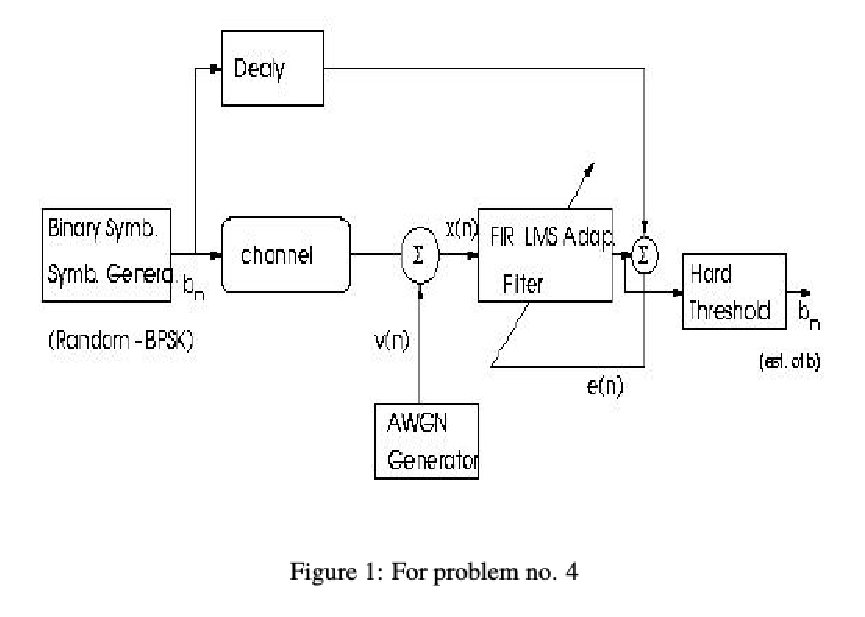
\includegraphics[width=\columnwidth]{./figs/figure3.eps}
\caption{}
\label{fig:figure3}
\end{figure}

\end{center}
\smallskip
and corrupted by additive white Gaussian noise (AWGN) with zero mean and variance $\sigma^2$. The delayed symbols that are fed at the output of the adaptive filter act as training signals.The channel impulse response is an 3-point FIR filter with a raised cosine type of structure.Parameter F controls the eigen value spread of $R=E[X(n)X^T(n)$.The structure of this problem is very similar to the one given in Haykin.\\
\medskip
Note:\\ 
\medskip
$$x(n)=\quad\sum_{k=1}^{3}h(k)b_{n-k}+v(n)$$\\
\medskip
You will need two random number generators; one for the symbols b n and the other for the AWGN.For AWGN assume $\sigma^2=0.01.$ For $b_n$ use a binary random number generator where 1 and -1 are generated with equal probability. You could do this by using a uniform random number generator, uniform over [−0.5, 0.5]. Whenever you get a negative number, set it to -1 and whenever you get a positive number set it to +1.
\medskip
\begin{enumerate}[(a)]
\item Experiment with different number of tap weights in the FIR LMS adaptive filter. For example you could consider 7, 9, or 11 tap weights.
\item Experiment with different variance for AWGN.
\item Estimate the amount of delay you need based on the number of tap weights you are using.
\item Run the experiment for two vales of $F$, say $F=3$ and $F=3.2$.
\item Plot the mean square error curves for each case.
\item Give a table for the values for $W(\infty).$
\item At the output of the adaptive filter have a hard threshold unit to classify the output as 1 or -1. This is done since we know that the transmitted symbols were 1 or -1. Now compute the percentage bits that are in error at convergence (this will give you the bit error rate (BER)).
\end{enumerate}
\medskip
\item Repeat the above channel equalization problem for the following cases:
\medskip
\begin{enumerate}[(a)]
\item The channel is no longer as given by the cosine function. But, now let the channel be modeled by an FIR filter of length 10, and each FIR coefficient be of unit magnitude. This way we will be considering the performance of the equalizer under a narrow band channel.
\item The data symbols are not binary (BPSK) but are QPSK. You can generalize the method used for generating BPSK to a method for generating QPSK. Plot the bit error rate. Do this for both the cases: (a) the FIR channel specified above, and (b) any other narrow band channel of your choice. Your channel could be FIR, IIR or non-linear.
\end{enumerate}
\end{enumerate}
\section{}
\begin{enumerate}
\item Implement Sato’s blind channel equalizer for:
\medskip
\begin{enumerate}[(a)]
\item BPSK data symbols and channel as specified\\
\bigskip
$h(n)=\begin{cases}
\bigskip
\frac{1}{2}[1+cos(\frac{2\pi}{F}{(n-2)})]& n=1,2,3\\
0 & otherwise
\end{cases}$\\
with $F=4.5$ or greater.
\item QPSK data, with the channel as above.
\item BPSK data, but with a narrow band channel
$h(n)=\begin{cases}
\bigskip
{1}&  n=0,1,... 9\\
0&  otherwise
\end{cases}$\\
\medskip
\item QPSK data with narrow band channel.
\item A channel of your choice.\\
In all cases specify the variance of additive noise.
\medskip
Compare the results of the Sato’s blind algorithm with the previous simulation where one had used the knowledge
of the channel.\\
\end{enumerate}
\medskip
\item Implement the \textit{Transform Based} LMS algorithm in the one step predictive mode. Use the data set for the LMS
algorithm from Home Work No.3, Problem 8. Use any real transform; DCT or DWT. Comment on the convergence
and MSE performance of the transform based LMS algorithm.
\end{enumerate}
%\bibliography{IEEEabrv,ee2340.bib}
\end{document}
